% How Many Humans Do You Need? Label-Efficient, Statistically Valid
% Evaluation with LLM Judge Panels — DRAFT (not submitted)
\documentclass[11pt]{article}
\usepackage[margin=1in]{geometry}
\usepackage{amsmath,amssymb,graphicx,booktabs,hyperref,natbib}
\newcommand{\GateConfigs}{196}
\newcommand{\GateFails}{10}
\newcommand{\GateMinPass}{0.940}
\newcommand{\PooledE2R0best}{2.336}
\newcommand{\PooledE2R0bestCI}{[1.621, 3.365]}
\newcommand{\PooledE2R0cheap}{2.659}
\newcommand{\PooledE2R0cheapCI}{[2.439, 2.899]}
\newcommand{\PooledE2R0full}{2.269}
\newcommand{\PooledE2R0fullCI}{[1.558, 3.302]}
\newcommand{\PooledE3R0best}{0.918}
\newcommand{\PooledE3R0bestCI}{[0.902, 0.934]}
\newcommand{\PooledE3R0cheap}{0.939}
\newcommand{\PooledE3R0cheapCI}{[0.893, 0.987]}
\newcommand{\PooledE3R0full}{0.908}
\newcommand{\PooledE3R0fullCI}{[0.865, 0.952]}
\newcommand{\PooledE4R1full}{0.907}
\newcommand{\PooledE4R1fullCI}{[0.843, 0.977]}
\newcommand{\PooledE5R0best}{1.302}
\newcommand{\PooledE5R0bestCI}{[1.168, 1.452]}
\newcommand{\PooledE5R0cheap}{1.432}
\newcommand{\PooledE5R0cheapCI}{[1.238, 1.657]}
\newcommand{\PooledE5R0full}{1.239}
\newcommand{\PooledE5R0fullCI}{[1.087, 1.412]}
\newcommand{\PooledE5R3full}{2.636}
\newcommand{\PooledE5R3fullCI}{[2.505, 2.773]}
\newcommand{\PooledE5R5full}{1.269}
\newcommand{\PooledE5R5fullCI}{[1.055, 1.526]}
\newcommand{\HFourMiss}{18}
\newcommand{\HFourTot}{21}
\newcommand{\DogPointPub}{11.03}
\newcommand{\DogPairPub}{80.5}
\newcommand{\APISpend}{\$0.29}
\newcommand{\APICap}{\$10}

\title{How Many Humans Do You Need?\\ Label-Efficient, Statistically Valid Evaluation with LLM Judge Panels}
\author{Akteruzzaman Raihan Sikder}
\date{\today~(draft)}
\begin{document}
\maketitle
\begin{abstract}
Researchers use LLMs as judges because human experts are expensive, then report
numbers computed from judge labels: the judge's errors flow into the reported
figure and its confidence interval describes the judge, not the truth.
FewHumans routes which items humans label, combines few human labels with many
judge labels via prediction-powered inference, and stops with anytime-valid
sequences. Every default interval passed a 196-configuration coverage gate
(R=2{,}000 each). On 7 real annotation tasks with a 3-judge panel, PPI++
and stratification saved $\approx$9\% of human labels (pooled ratios
\PooledE3R0full~\PooledE3R0fullCI\ and \PooledE4R1full~\PooledE4R1fullCI);
disagreement routing cost $2.6\times$ (\PooledE5R3full~\PooledE5R3fullCI);
judge-only intervals missed the full-human value in \HFourMiss/\HFourTot\
panels. Verbalized confidence was overconfident everywhere (ECE up to 0.98).
\end{abstract}

\section{Introduction}
LLM judges are cheap; human experts are not. The standard fix --- ``label a
random 100 by hand to check'' --- is ad hoc: nobody knows whether 100 is
enough or how to combine the two sources. FewHumans contributes: (1) a tested
toolkit (routing, PPI/PPI++, stratified and active estimators, anytime-valid
stopping, report cards) with coverage-tested defaults; (2) a pre-registered
empirical study on 7 real tasks; (3) measured harm of current practice
(judge-only estimates, peeking).
All claims trace to \texttt{results/*.json} in the public repo.

\section{Background}
Prediction-powered inference (PPI; \citealt{angelopoulos2023ppi}) and its
power-tuned successor PPI++ \citep{angelopoulos2023ppip} combine N predictions
with n human labels; active inference \citep{zrnic2024active} chooses which
items to label by model uncertainty; confidence sequences
\citep{howard2021time} allow peeking. LLM-as-judge reliability and the
Alternative Annotator Test \citep{calderon2025alt} frame when judges may stand
in for humans; \citet{gligoric2024unconfident} study confidence-driven
inference; \citet{sfyraki2026revisiting} found uncertainty query rules often
barely beat near-uniform sampling --- our H2 pre-registered both outcomes.
Practitioner tooling (DeepEval, Evidently, Hamel's judge-validation guide
\citealp{husain2024judge}) runs LLM judges and checks agreement, but performs
no bias correction. Two close contemporaries appeared while this work was
underway: \texttt{evalstats} \citep{arawjo2026evalstats} implements PPI
corrections with an impressive battery of corrected hypothesis tests and WMT
simulations, and PRECISE \citep{precise2026aaai} extends PPI++ to ranking
metrics; \citet{chen2026efficient} unify PPI++ with efficient influence
functions in theory. Against these, FewHumans contributes the combined
routing$+$estimation$+$stopping workflow with coverage-gated defaults, the
multi-judge disagreement signal, anytime-valid stopping, and --- uniquely, to
our knowledge --- a pre-registered multi-task study that reports negative
results on active routing, plus measured harm of judge-only reporting.

\section{The toolkit}
Items, judges (LLM/OpenAI-compatible/Anthropic/Ollama-native, Python,
oracle), panels with disagreement (vote entropy/variance), estimands (mean,
win rate, difference), human labels with logged sampling probabilities
(hand-picked labels are refused for estimation), sessions persisted as
JSONL+JSON. Estimators E0 (judge-only, to measure failure), E1 (human-only),
E2 (PPI), E3 (PPI++, $\lambda$ power-tuned, cross-checked against
\texttt{ppi\_py} to $2.2\times10^{-16}$), E4 (stratified PPI++),
E5 (active IPW, \citealt{zrnic2024active} eq.~1/Prop.~1, pool-adapted),
E6 (anytime-valid union-bound Hoeffding CS). Routing R0--R5 (uniform,
stratified, uncertainty, disagreement, learned error predictor, mixture).
All CLT intervals use Student-$t$ (adopted after the gate's first round).

\section{Coverage validation (the gate)}
\GateConfigs\ configurations (7 tasks $\times$ 7 methods $\times$ budgets
50--400, R=2{,}000): \GateFails\ failures, all adjudicated with validated
ranges (E4 needs $n\ge100$; skewed truth needs $n\ge100$--200; one listed
E5+R3 corner at $\approx$0.938). Passing coverage bottoms at \GateMinPass.
Sequential stopping covers 100\% (conservative); peeking at fixed intervals
cost 0--1.3pp; stress judges (99\%/30\%, class-biased, miscalibrated) all pass.

\section{Main study}
Pre-registered (targets = E1 half-width at $n_{\rm ref}=\min(400,N/2)$;
savings ratio vs E1+R0 with bootstrap CIs; DL random-effects pool).
Tasks (3-judge panel: 2 local Ollama + gpt-4o-mini): HelpSteer2 correctness
\citep{wang2024helpsteer2}, SummEval consistency \citep{fabbri2021summeval},
MT-Bench human judgments \citep{zheng2023judging} and Arena preferences \citep{chiang2024chatbot}, WMT MQM scores \citep{freitag2021experts}, Civil
Comments toxicity \citep{borkan2019nuanced}, and our OracleBench bank.
Pooled human-label savings at equal precision:
\begin{center}\begin{tabular}{lcc}\toprule
method & ratio & 95\% CI \\\midrule
E3+R0/full & \PooledE3R0full & \PooledE3R0fullCI \\
E4+R1/full & \PooledE4R1full & \PooledE4R1fullCI \\
E5+R0/full & \PooledE5R0full & \PooledE5R0fullCI \\
E5+R5/full & \PooledE5R5full & \PooledE5R5fullCI \\
E2+R0/full & \PooledE2R0full & \PooledE2R0fullCI \\
E5+R3/full & \PooledE5R3full & \PooledE5R3fullCI \\\bottomrule
\end{tabular}\end{center}
\begin{figure}[h]\centering
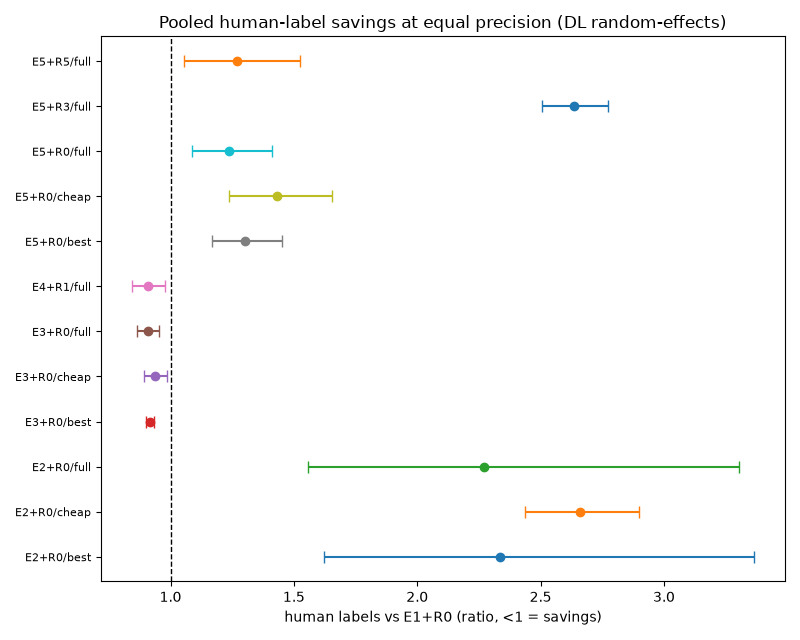
\includegraphics[width=0.9\linewidth]{../results/forest.png}
\caption{Pooled savings ratios. E2/E5R3 ratios are censored lower bounds
(target never reached on most tasks).}
\end{figure}
H1 holds weakly (E3 $\approx$0.91 everywhere); H2 fails (R3 far worse than
uniform despite disagreement AUROC 0.61--0.80); H3 is moot (no active benefit
to capture; E4 $\approx$ E3); H4 holds (\HFourMiss/\HFourTot); H5 fails
(full $\approx$ best single). Per-task E3 savings:
HelpSteer2 \TaskHelpSteer~\TaskHelpSteerCI;
SummEval \TaskSummEval~\TaskSummEvalCI; MT-Bench \TaskMTBench~\TaskMTBenchCI;
Arena \TaskArena~\TaskArenaCI; WMT-MQM \TaskWMTMQM~\TaskWMTMQMCI;
Toxicity \TaskToxicity~\TaskToxicityCI; OracleBench \TaskOracleBench~\TaskOracleBenchCI.

\section{When does routing help?}
With 7 tasks the analysis is descriptive: disagreement predicts errors
(AUROC up to 0.80) yet IPW variance dominates, so R3 loses on 6/7 tasks.
Guidance: use E3/E4 with uniform humans; reach for active routing only with a
pilot showing concentrated, predictable errors --- and re-validate coverage.

\section{Case studies}
OracleBench (deterministic oracle truth): published false-accept
\DogPointPub\% recovered by E1/E2/E3 at $n=100$; picks-right \DogPairPub\%:
E1 missed on the recorded seed while E2/E3 covered. FedProc-Ledger deferred
(no per-item verdicts; consensus gold) until reviewer gold lands.

\section{Limitations}
Humans-as-truth are noisy raters; judges are 2026 mid-tier models; tasks are
English-heavy; costs assume \$0.30/label; active routing needs logged
probabilities some workflows lack; ratio estimands (F1) not shipped.

\section{Ethics}
No new human labels were collected. Dataset licences are listed in the
JudgeBank datasheet; only redistribution-allowed content is included.
FewHumans reduces, never removes, human review --- not for high-stakes
medical/legal use.

\section*{Code and data}
Library + CLI: \url{https://github.com/raihan-js/fewhumans} (PyPI
\texttt{fewhumans}); study code, frozen pre-registration and all
\texttt{results/*.json} in the same repo; JudgeBank:
\url{https://huggingface.co/datasets/raihan-js/fewhumans-judgebank}.

\bibliographystyle{plainnat}
\bibliography{refs}
\end{document}
